\chapter{Methodology}
\label{ch:methodology}

\section{Introduction}

This chapter presents the methodology and system analysis adopted for the design and development of Echora, an AI-powered sensory substitution system for Blind and Low Vision (BLV) users. It describes the structured approach used to transform project objectives and user needs into a coherent technical solution, ensuring feasibility, usability, and alignment with real-world constraints.

The chapter outlines the overall development methodology, including the rationale behind key design decisions, the validation of project relevance through proof of interest, and the planning strategies employed to manage complexity and risk. Emphasis is placed on iterative development, user-centered design principles, and continuous evaluation to ensure that the system effectively supports both macro-navigation and micro-interaction tasks.

In addition, this chapter details the project planning process, including the project management plan and the adoption of Agile practices. These practices enable flexibility, incremental progress, and early integration of feedback, which are critical for developing a real-time, safety-critical assistive system such as Echora. Together, the methodology and planning framework described in this chapter provide a solid foundation for the system design, implementation, and evaluation discussed in subsequent sections.

\section{Methodology}

The development of the Echora system follows a user-centered, iterative methodology that combines principles from systems engineering, human-centered design, and Agile software development. This methodology is selected to address the technical complexity, real-time constraints, and safety-critical nature of assistive technology for Blind and Low Vision (BLV) users.

At the core of this methodology is the transformation of user needs into functional system components through continuous validation and refinement. Rather than treating navigation, object interaction, and perception as isolated problems, Echora is developed as an integrated sensory substitution system in which sensing, processing, and feedback are tightly coupled.

The methodology begins with requirements analysis grounded in user-centered design. The development process starts by analyzing user needs, accessibility requirements, and limitations of existing assistive technologies. Functional and non-functional requirements are derived from the challenges faced by BLV users in navigation and object interaction, from safety, usability, and accessibility considerations, and from insights obtained through related research and market analysis. These requirements guide subsequent design and implementation decisions, ensuring that system development remains focused on real-world usability rather than purely technical performance.

Following requirement definition, Echora is decomposed into independent yet interconnected modules to support modular system engineering. The system is structured around sensor acquisition and synchronization across depth, RGB, and inertial inputs, perception and AI processing for mapping, detection, and recognition, context-awareness and mode switching between navigation and interaction, and feedback generation through spatial audio and haptics. This modular architecture enables components to be developed, tested, and optimized independently while maintaining a clear pathway toward scalable system integration.

After modularization, development proceeds through iterative prototyping and incremental implementation. The system is built through successive prototypes, where each iteration introduces a limited set of features---such as navigation audio, hand guidance, or text recognition---that are tested individually before integration into the full system. This approach enables early identification of performance bottlenecks, usability concerns, and sensor limitations. Feedback from testing and evaluation is used to refine system behavior, improve feedback strategies, and optimize real-time performance.

A core methodological principle in Echora is multimodal sensor fusion combined with real-time on-device processing. Depth, vision, inertial data, and other sensing signals are integrated to construct a unified perception of the environment. Processing is performed entirely on-device to satisfy latency constraints, protect user privacy, and improve system reliability in environments without stable connectivity. Real-time constraints are treated as an explicit design requirement throughout development, and latency, frame rate, and resource usage are monitored continuously to ensure responsive and safe operation.

The methodology also emphasizes feedback design and cognitive load management. Audio and haptic feedback are designed to be intuitive and non-overlapping, with information prioritized by urgency and context. Critical safety alerts are designed to override non-essential feedback when necessary. In addition, automatic mode switching reduces cognitive load by activating only the system functions relevant to the user’s current context, enabling smoother transitions between macro-navigation and micro-interaction.

Validation and risk mitigation are integrated across the entire development lifecycle rather than being deferred to a final evaluation stage. Individual modules are validated independently through unit-level tests, followed by system-level integration testing to confirm correct end-to-end behavior. Potential risks, including sensor failure, latency spikes, or feedback overload, are addressed through fallback behaviors and graceful degradation strategies that maintain safety and usability even under degraded conditions.

Through this structured yet flexible methodology, Echora is developed as a reliable, adaptive, and user-focused assistive system capable of operating effectively in complex real-world environments.

\subsection{Proof of Interest}

\begin{figure}[H]
    \centering
    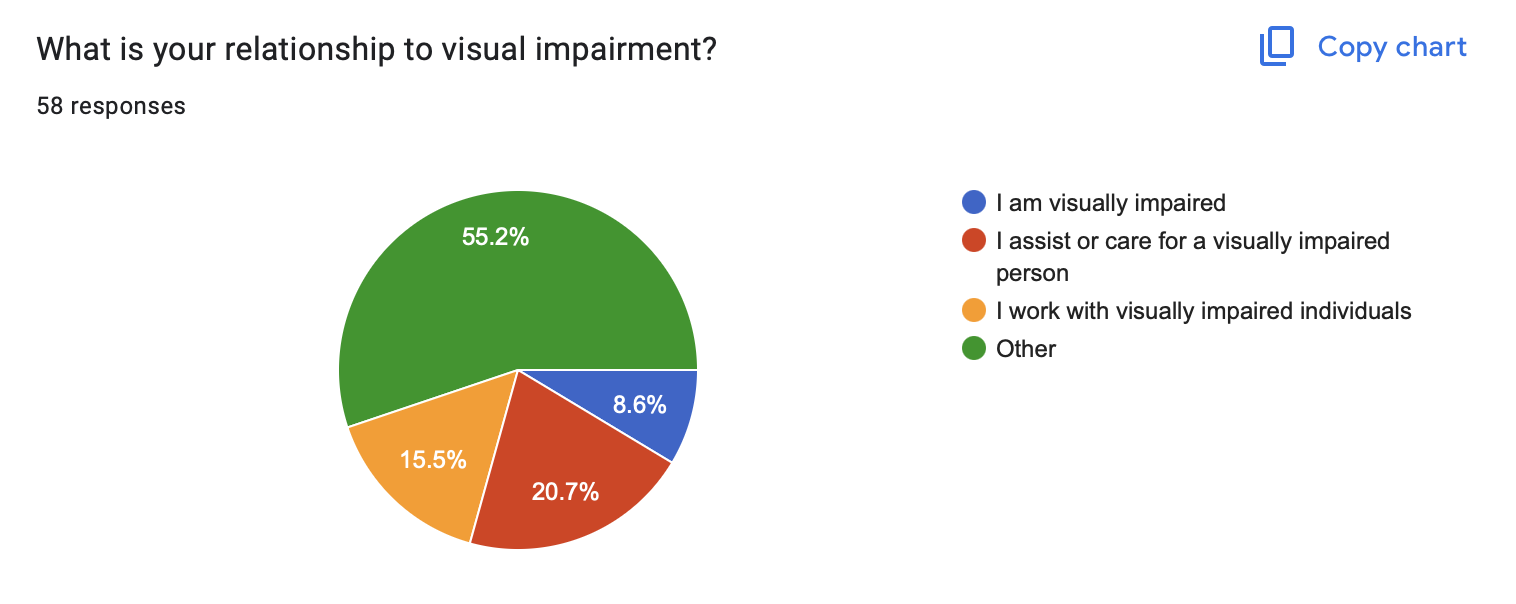
\includegraphics[width=0.8\textwidth]{assets/1.png}
    \hfill
    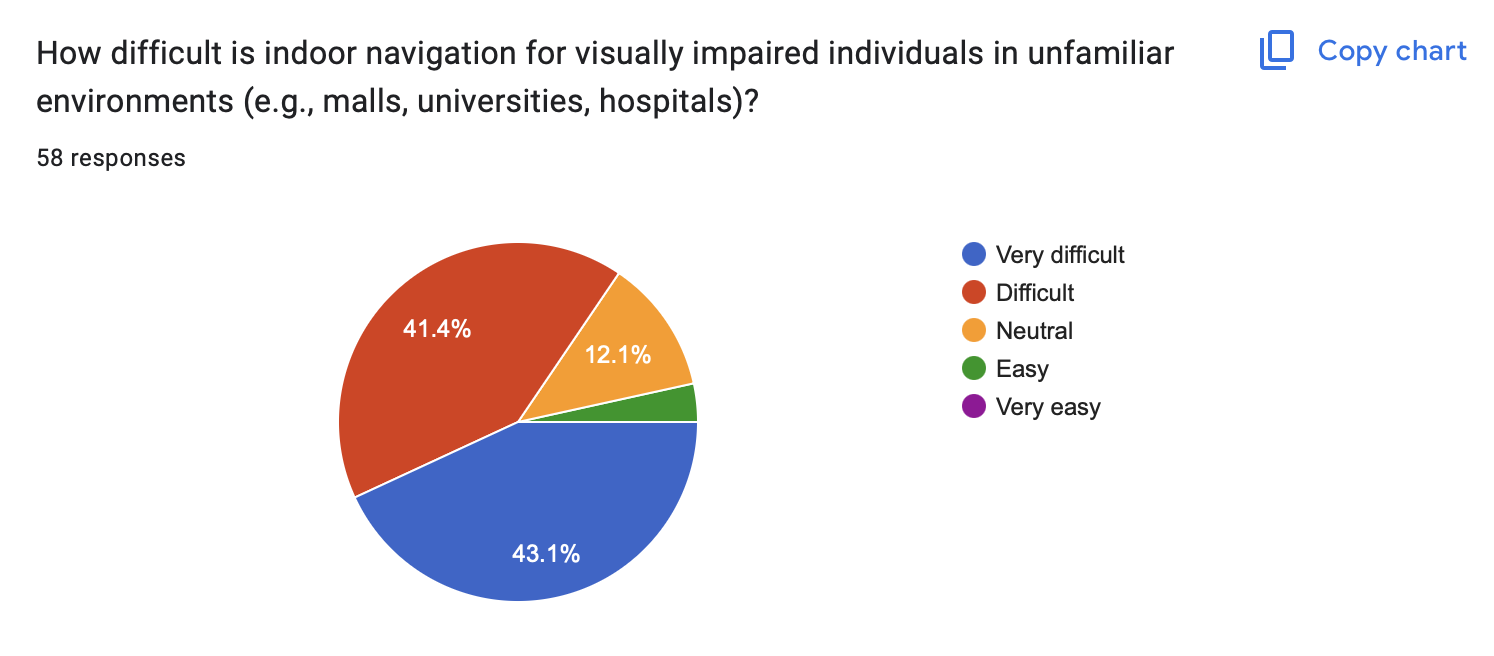
\includegraphics[width=0.8\textwidth]{assets/2.png}
    \caption{Questionnaire Statistics Graphs 1 \& 2}
    \label{fig:poi_1_2}
\end{figure}

\begin{figure}[H]
    \centering
    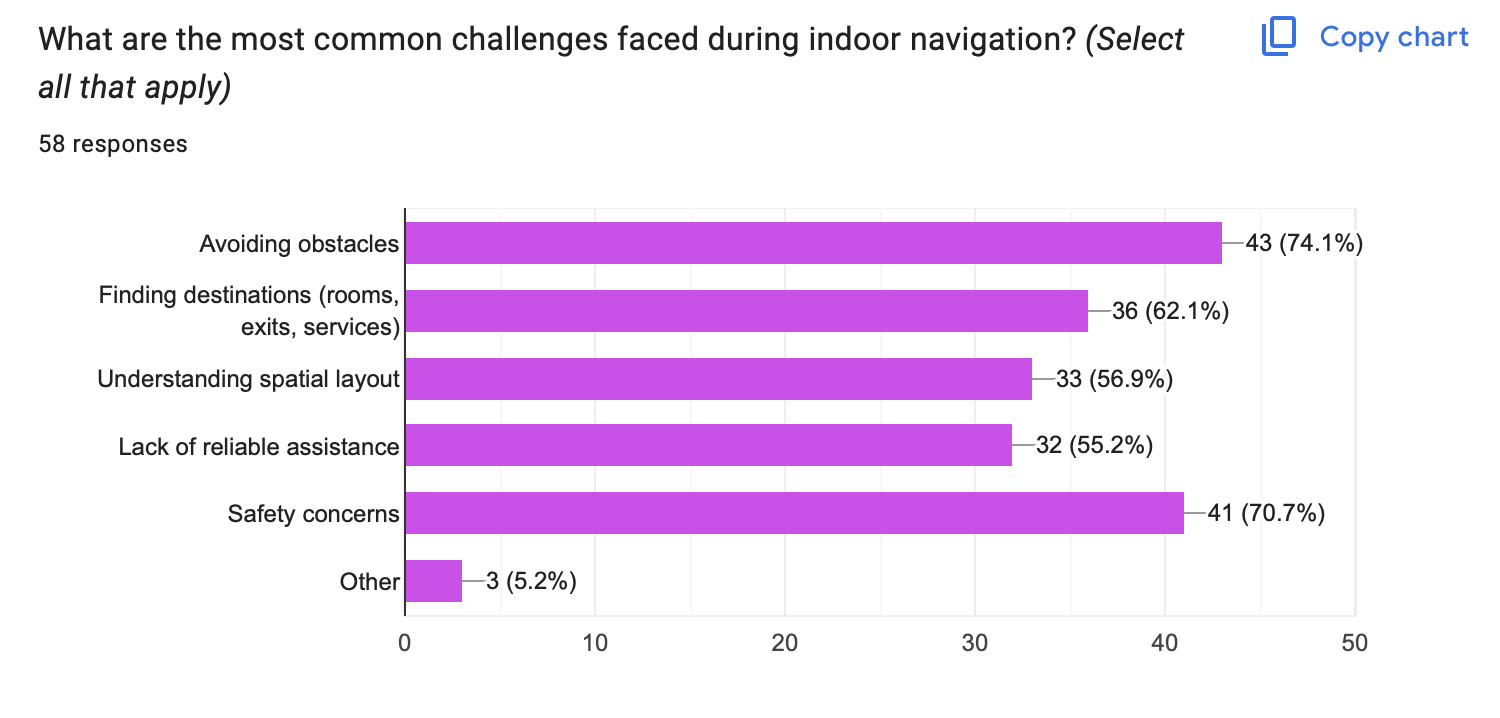
\includegraphics[width=0.8\textwidth]{assets/3.png}
    \hfill
    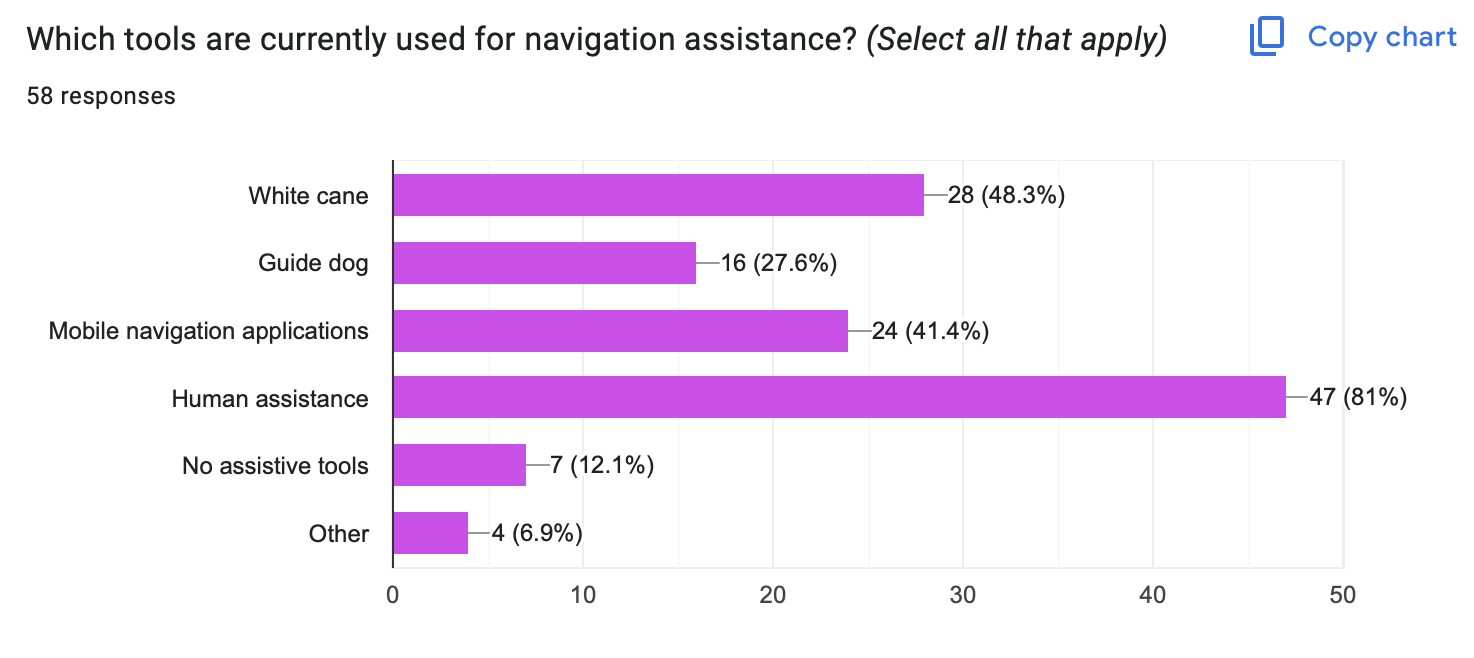
\includegraphics[width=0.8\textwidth]{assets/4.png}
    \caption{Questionnaire Statistics Graphs 3 \& 4}
    \label{fig:poi_3_4}
\end{figure}

\begin{figure}[H]
    \centering
    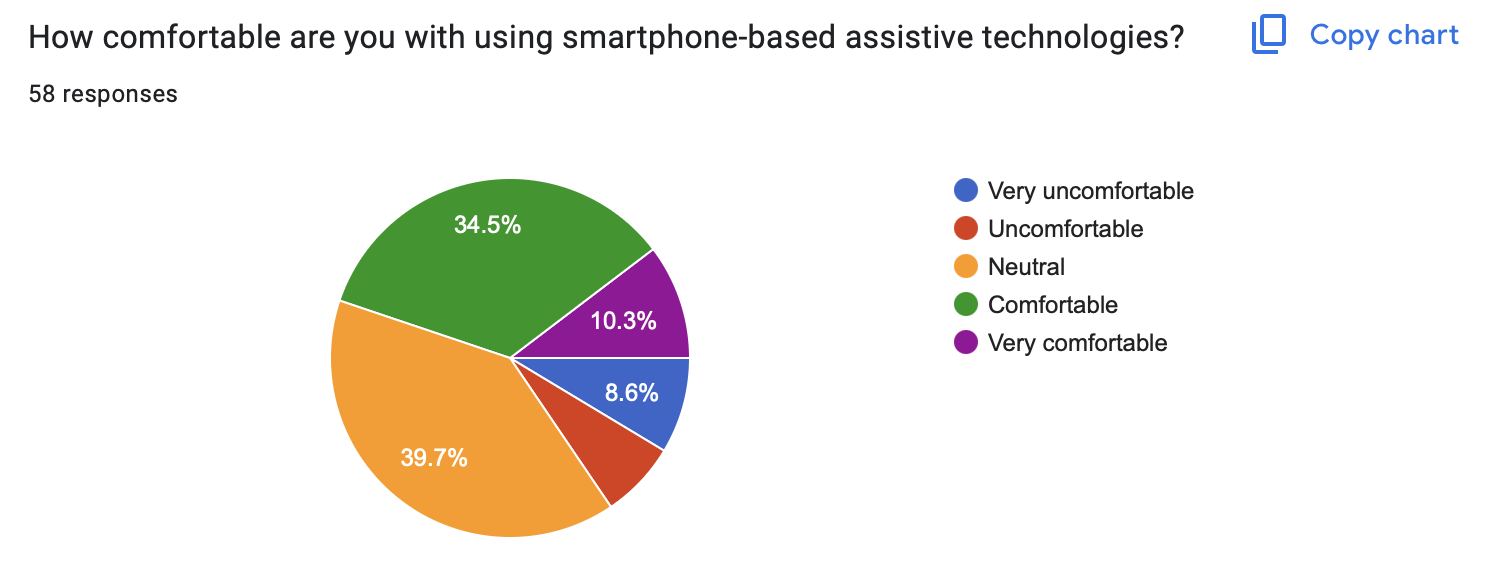
\includegraphics[width=0.8\textwidth]{assets/5.png}
    \hfill
    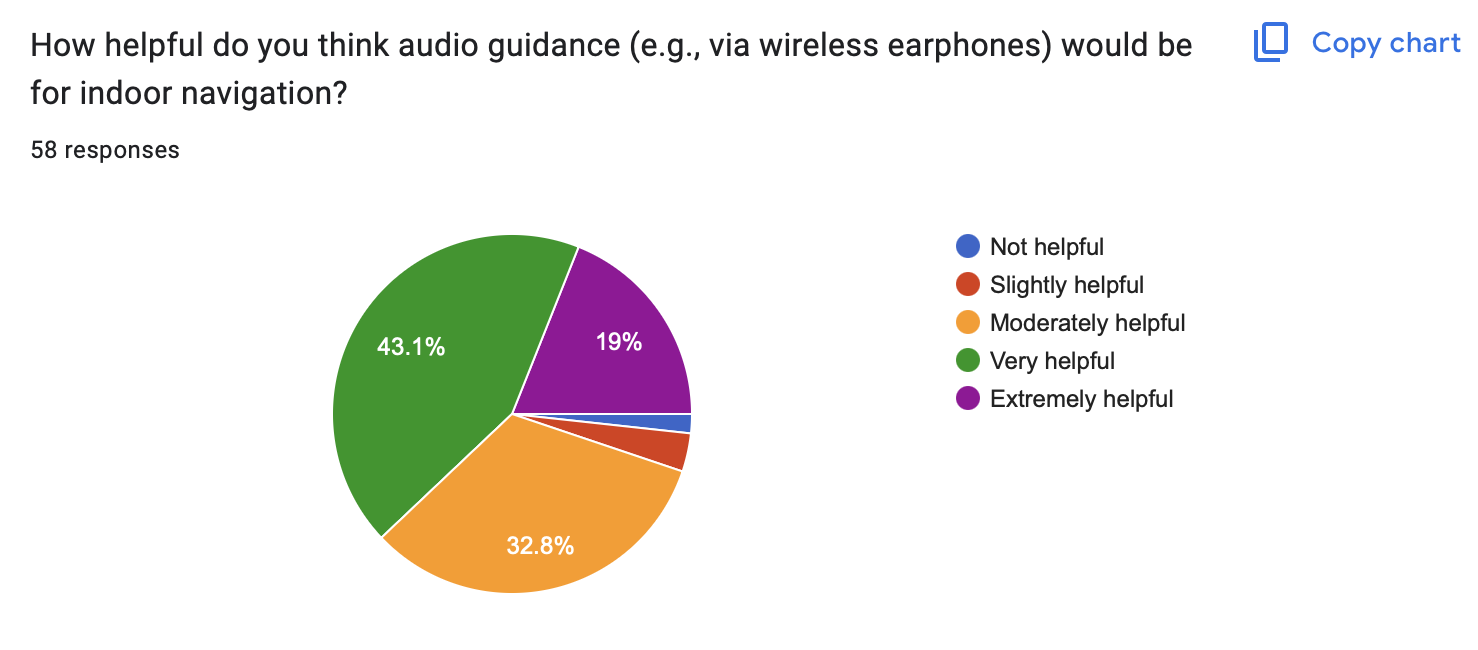
\includegraphics[width=0.8\textwidth]{assets/6.png}
    \caption{Questionnaire Statistics Graphs 5 \& 6}
    \label{fig:poi_5_6}
\end{figure}

\begin{figure}[H]
    \centering
    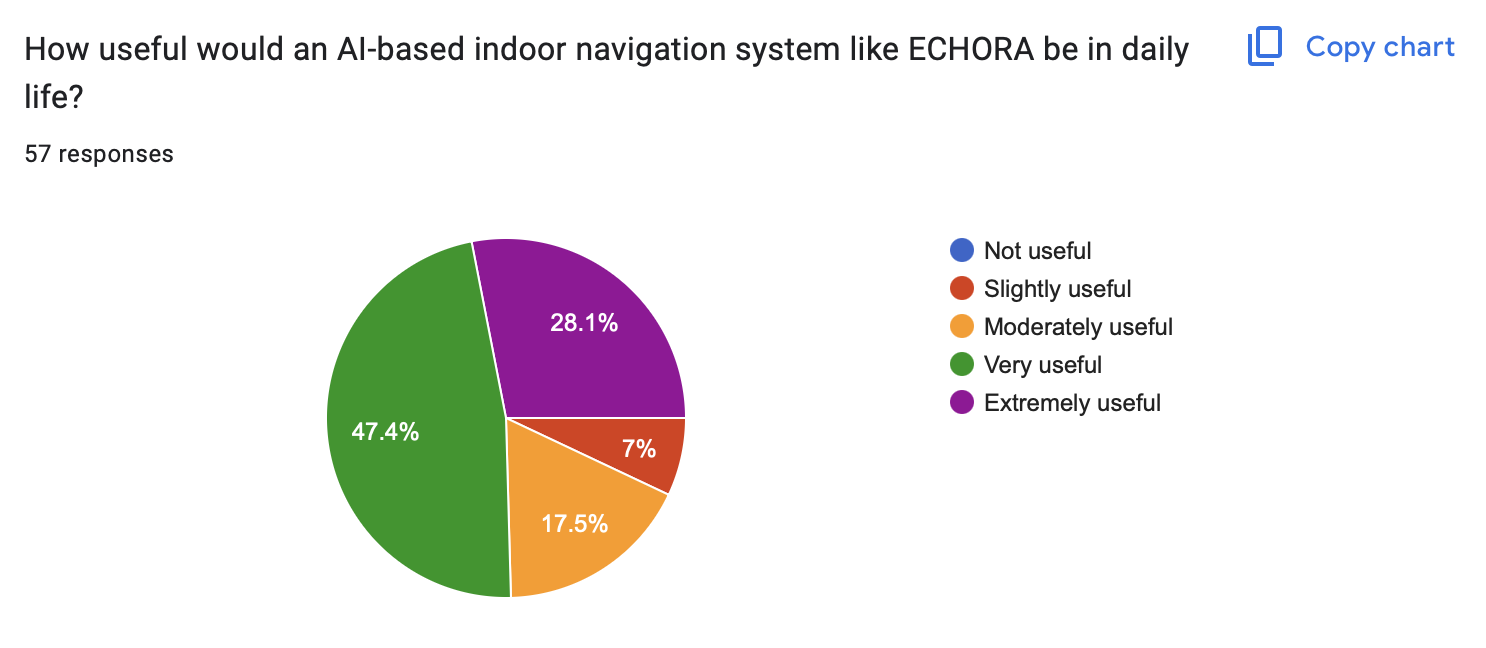
\includegraphics[width=0.8\textwidth]{assets/7.png}
    \hfill
    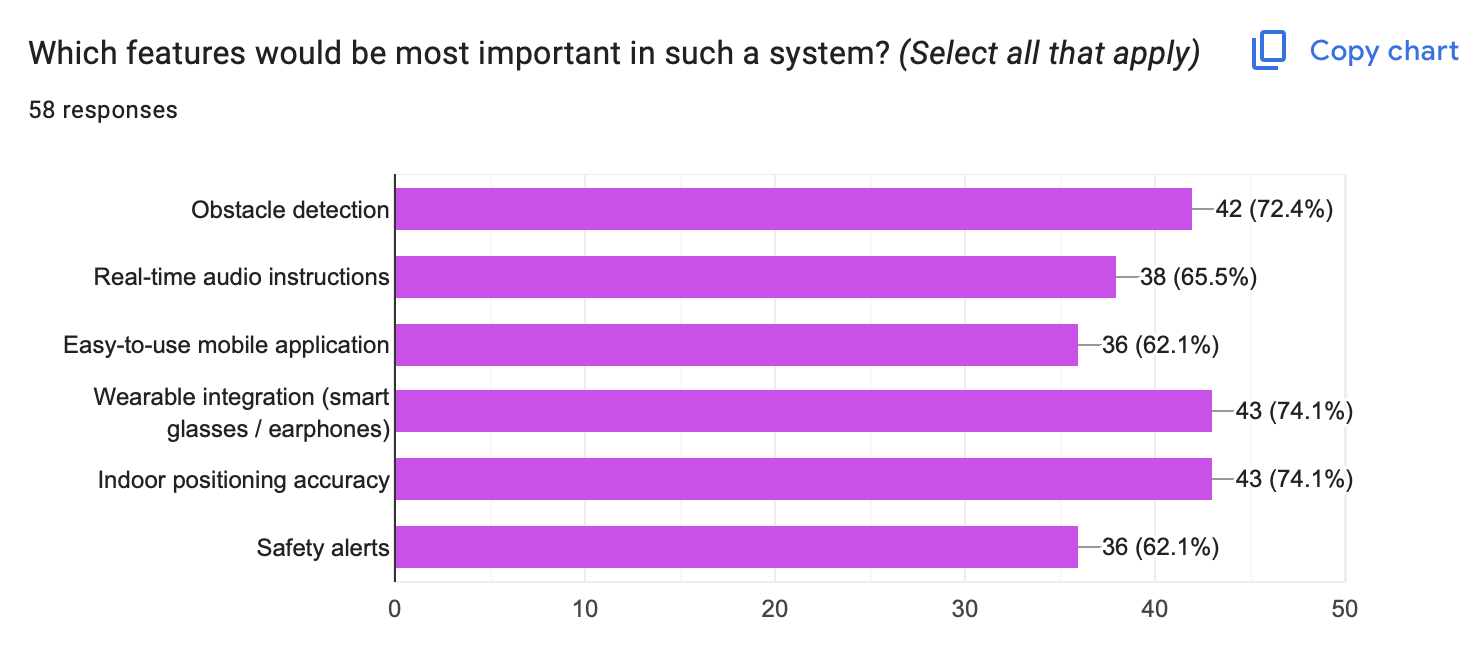
\includegraphics[width=0.8\textwidth]{assets/8.png}
    \caption{Questionnaire Statistics Graphs 7 \& 8}
    \label{fig:poi_7_8}
\end{figure}

\begin{figure}[H]
    \centering
    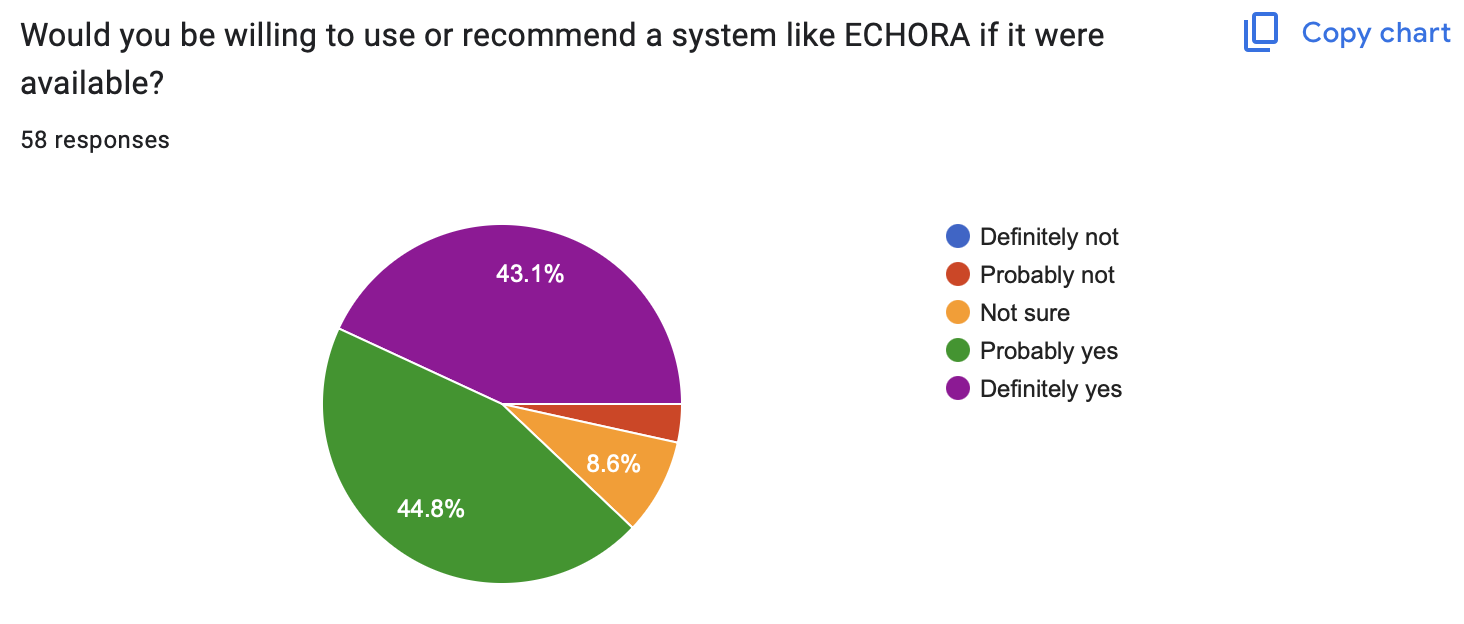
\includegraphics[width=0.8\textwidth]{assets/9.png}
    \hfill
    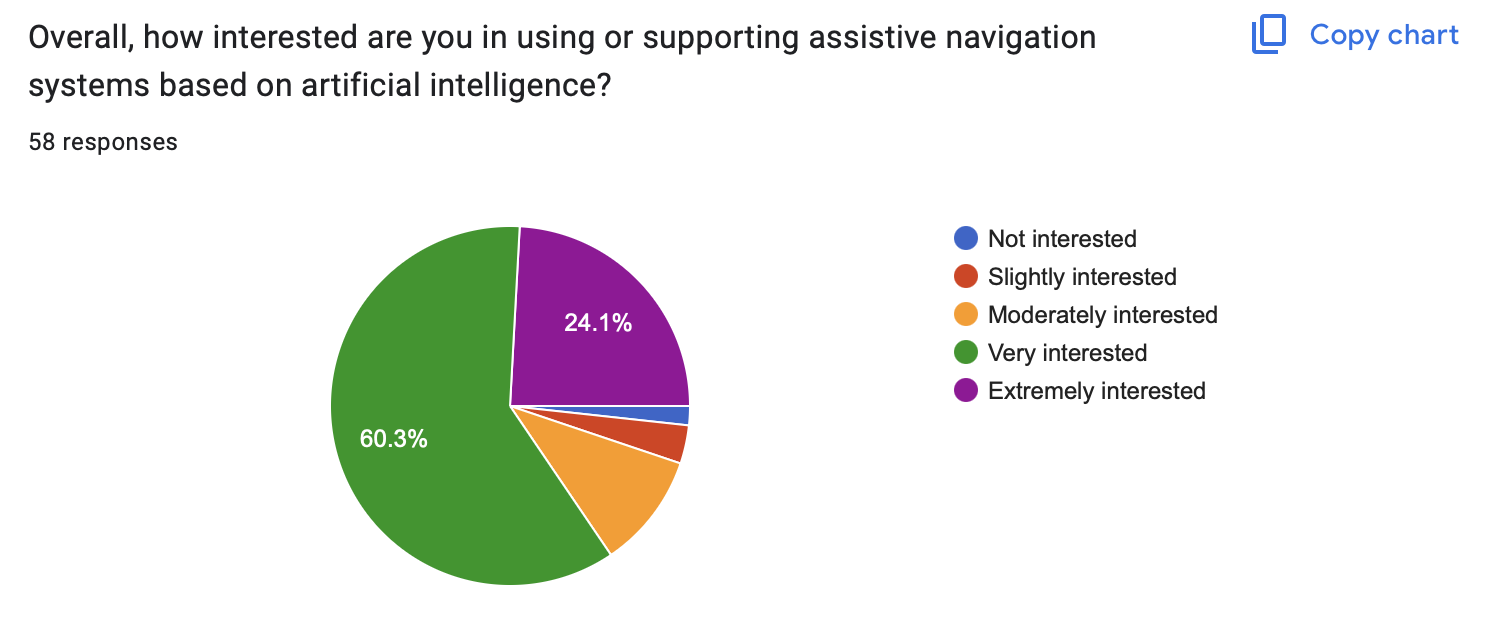
\includegraphics[width=0.8\textwidth]{assets/10.png}
    \caption{Questionnaire Statistics Graphs 9 \& 10}
    \label{fig:poi_9_10}
\end{figure}

\newpage
\section{Project Planning}

\subsection{Project Management Plan}

\begin{table}[H]
\raggedright
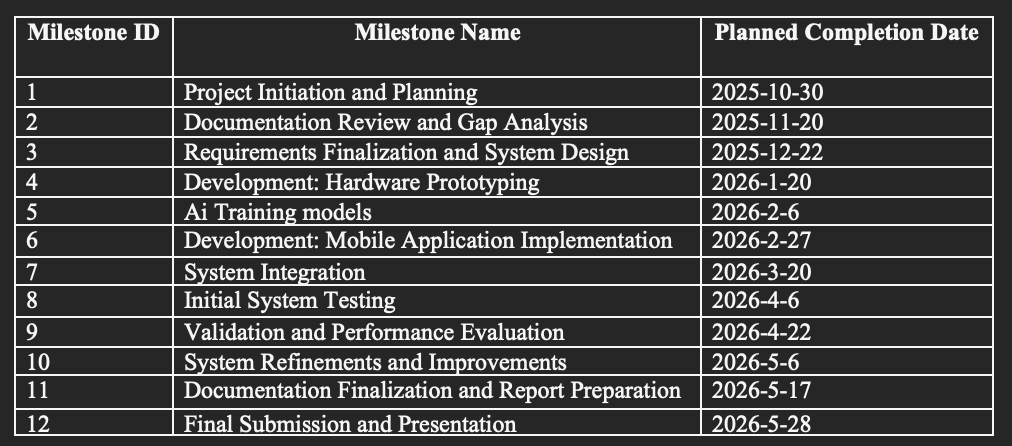
\includegraphics[height=0.5\textwidth]{assets/Table Project Milestone.png}
\caption{Project Milestone Table}
\label{tab:milestones}
\end{table}

\begin{table}[H]
\raggedright
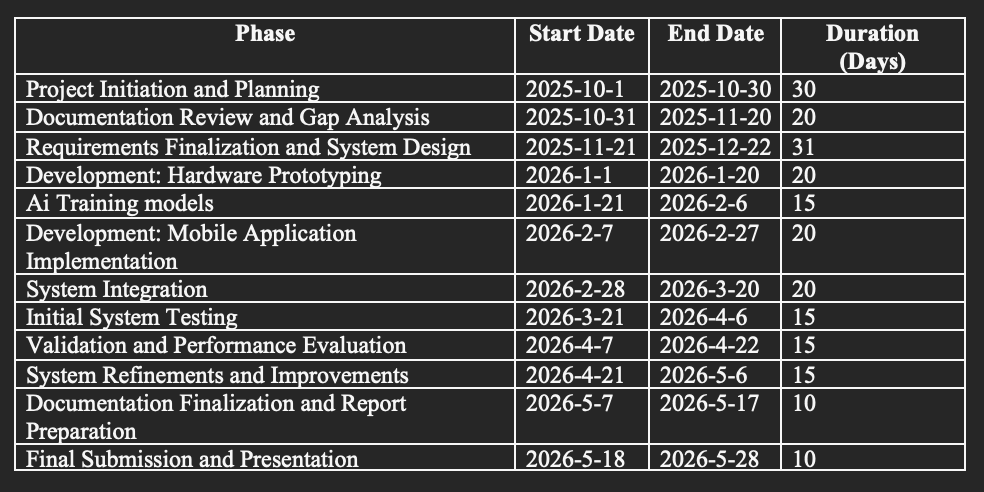
\includegraphics[height=0.55\textwidth]{assets/Table Project TimeLine.png}
\caption{Project Timeline Table}
\label{tab:timeline}
\end{table}

\newpage
\subsection{Agile Project Planning}

The Echora project adopts Agile practices to support incremental development, early validation, and continuous adaptation to technical and usability feedback. Agile planning is used to break down complex system requirements into manageable tasks, enabling iterative delivery of system components and improved visibility of progress across documentation and implementation phases. Sprint-based execution supports frequent integration and testing, reducing the likelihood of late-stage integration failures and enabling earlier identification of performance and feasibility risks.

The Agile workflow is managed using a backlog-driven process in which tasks are prioritized based on implementation dependencies, risk level, and expected user impact. The documentation phase backlog is used to organize requirement definition, system specification, and design deliverables, while the implementation phase backlog is used to track development, integration, testing, and optimization tasks. Sprint planning and reviews provide a structured mechanism for assessing progress, updating priorities, and integrating lessons learned into subsequent iterations.

\begin{figure}[H]
\raggedright
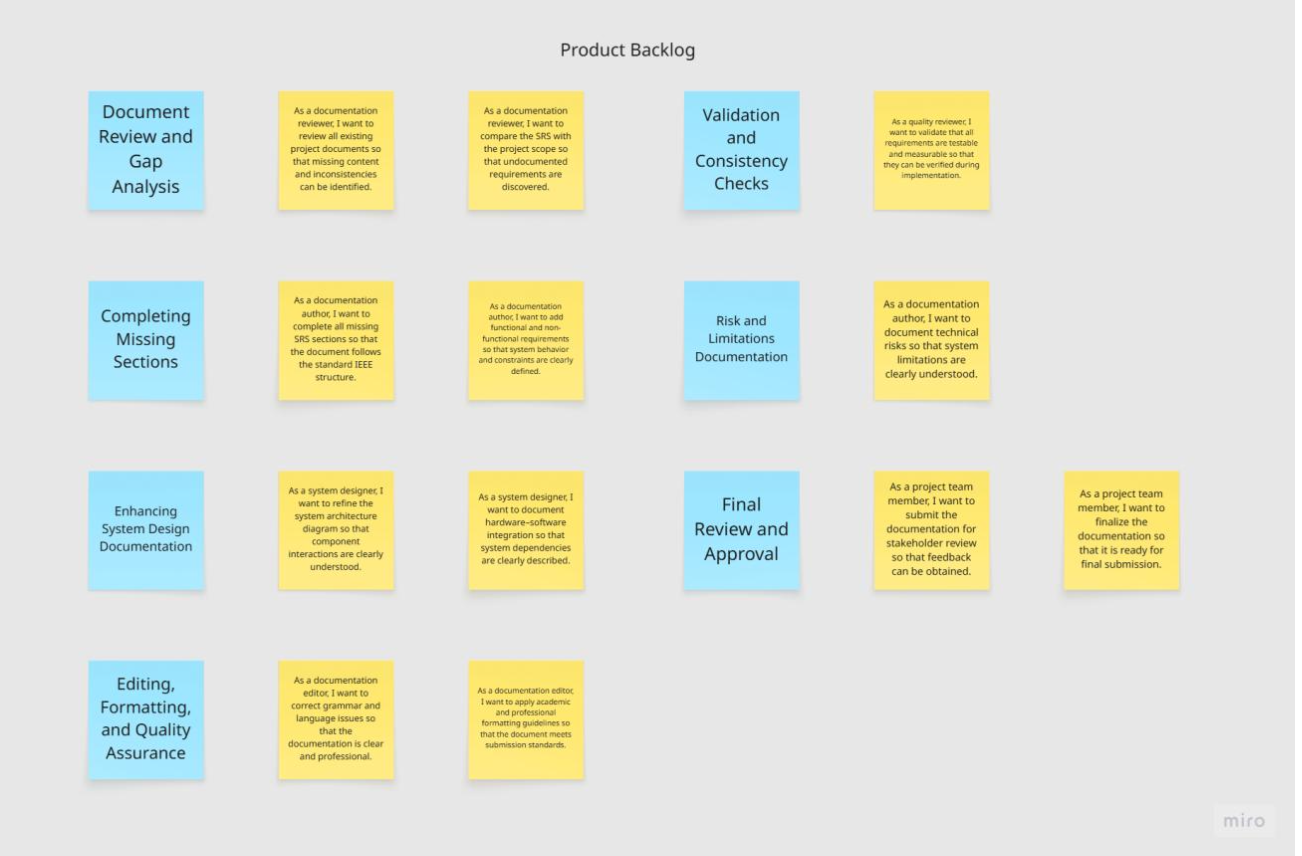
\includegraphics[height=0.73\textwidth]{assets/agile/doc phase.png}
\caption{Documentation Phase Backlog}
\label{fig:agile_doc_backlog}
\end{figure}

\begin{figure}[H]
\raggedright
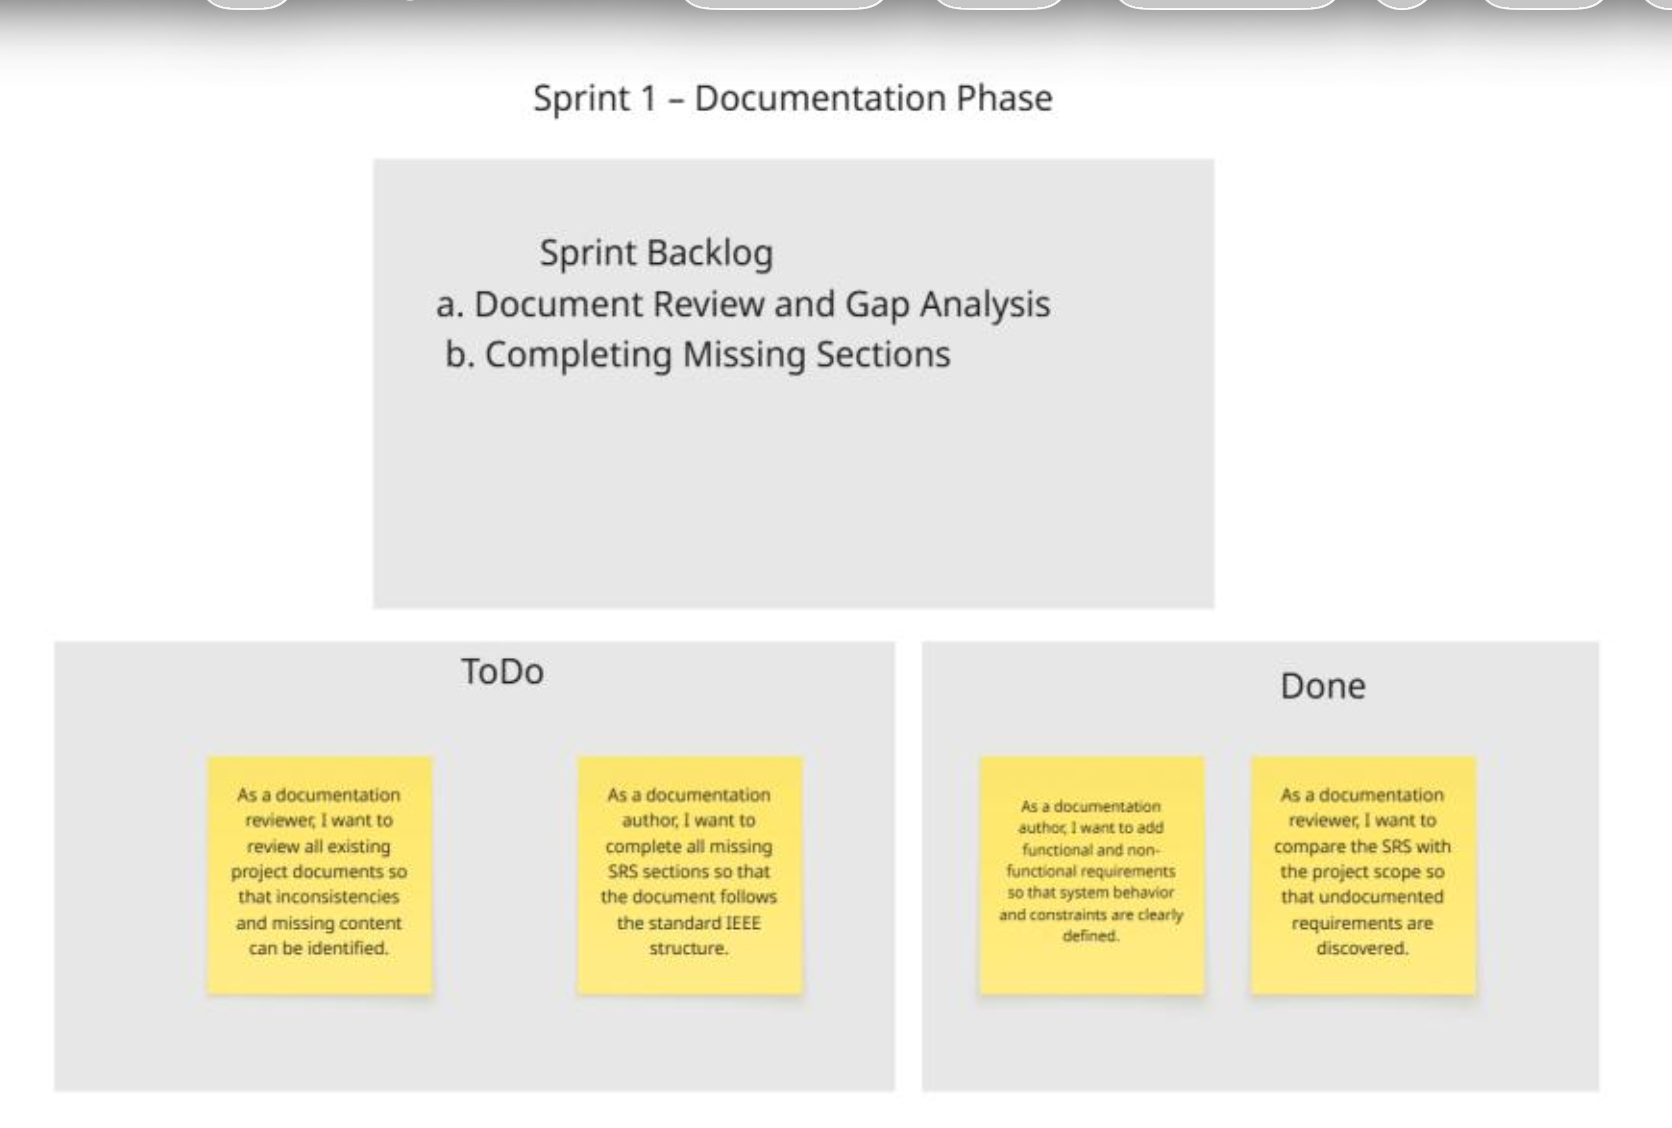
\includegraphics[height=0.6\textwidth]{assets/agile/s1 doc phase.png}
\caption{Sprint 1 Documentation Phase}
\label{fig:agile_doc_s1}
\end{figure}

\begin{figure}[H]
\raggedright
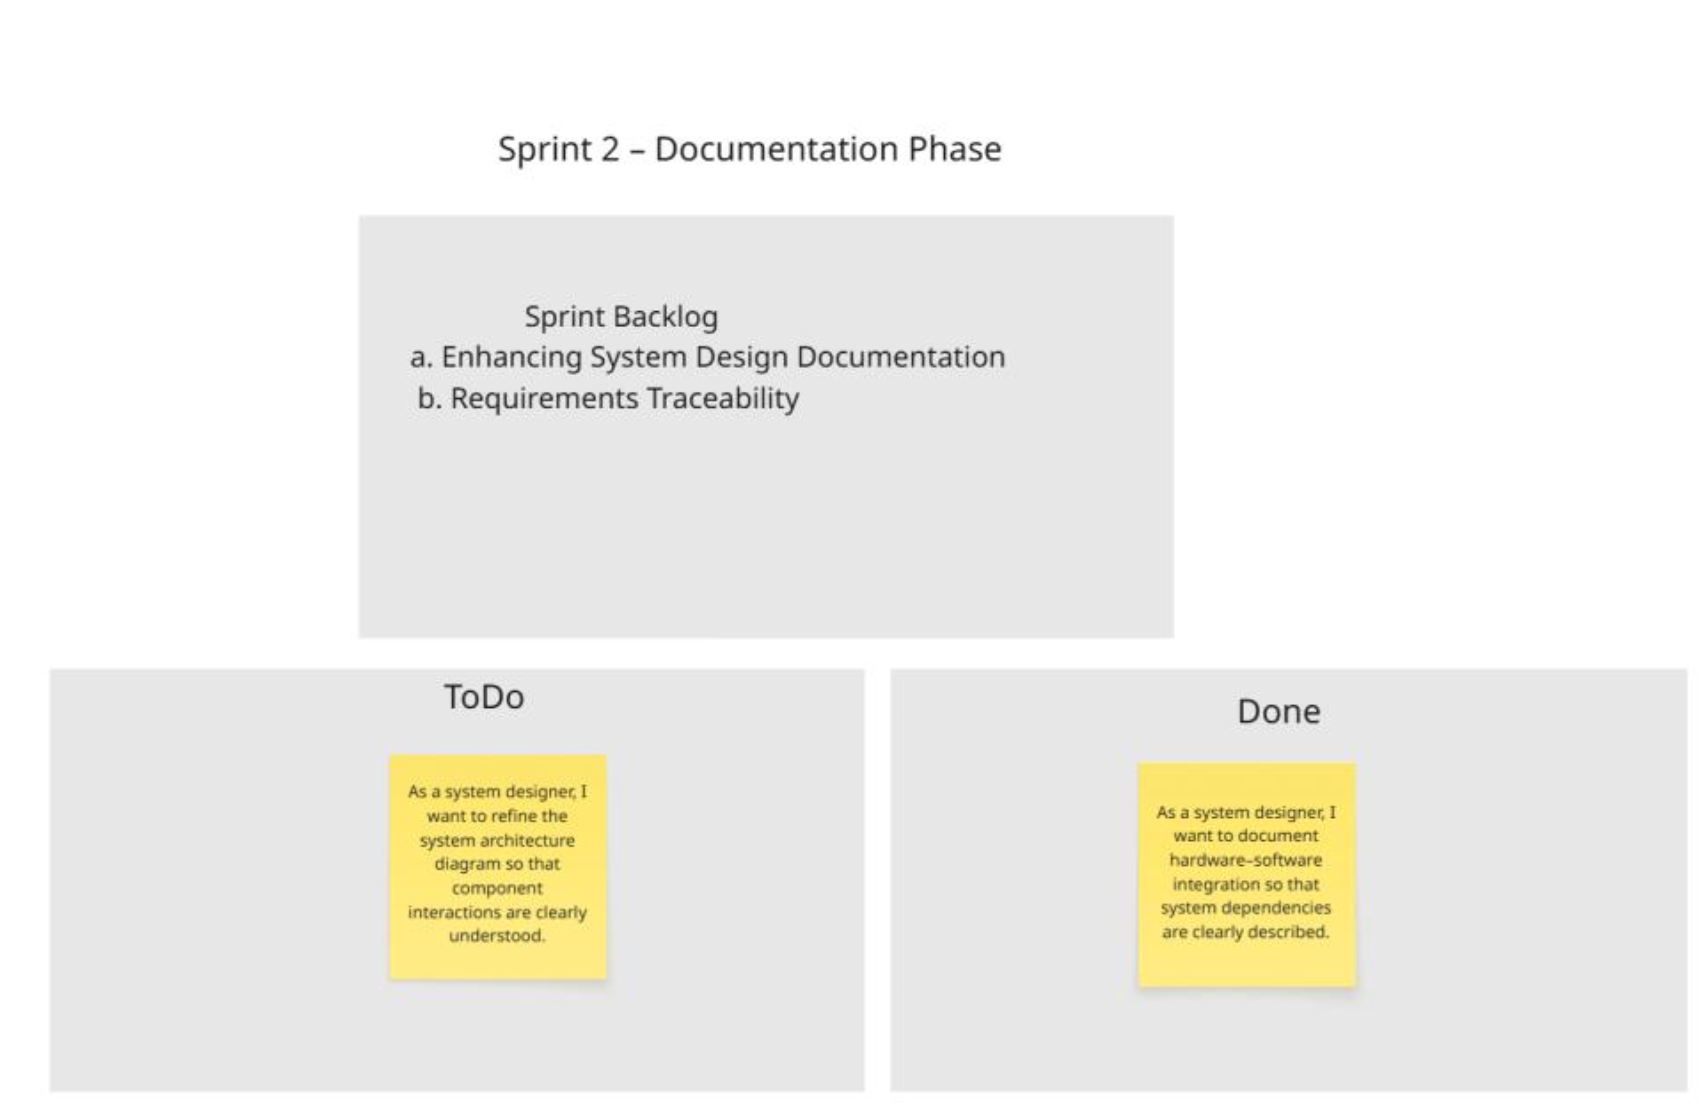
\includegraphics[height=0.6\textwidth]{assets/agile/s2 doc phase.png}
\caption{Sprint 2 Documentation Phase}
\label{fig:agile_doc_s2}
\end{figure}

\begin{figure}[H]
\raggedright

\includegraphics[height=0.6\textwidth]{assets/agile/s3 doc phase.png}
\caption{Sprint 3 Documentation Phase}
\label{fig:agile_doc_s3}
\end{figure}

\begin{figure}[H]
\raggedright
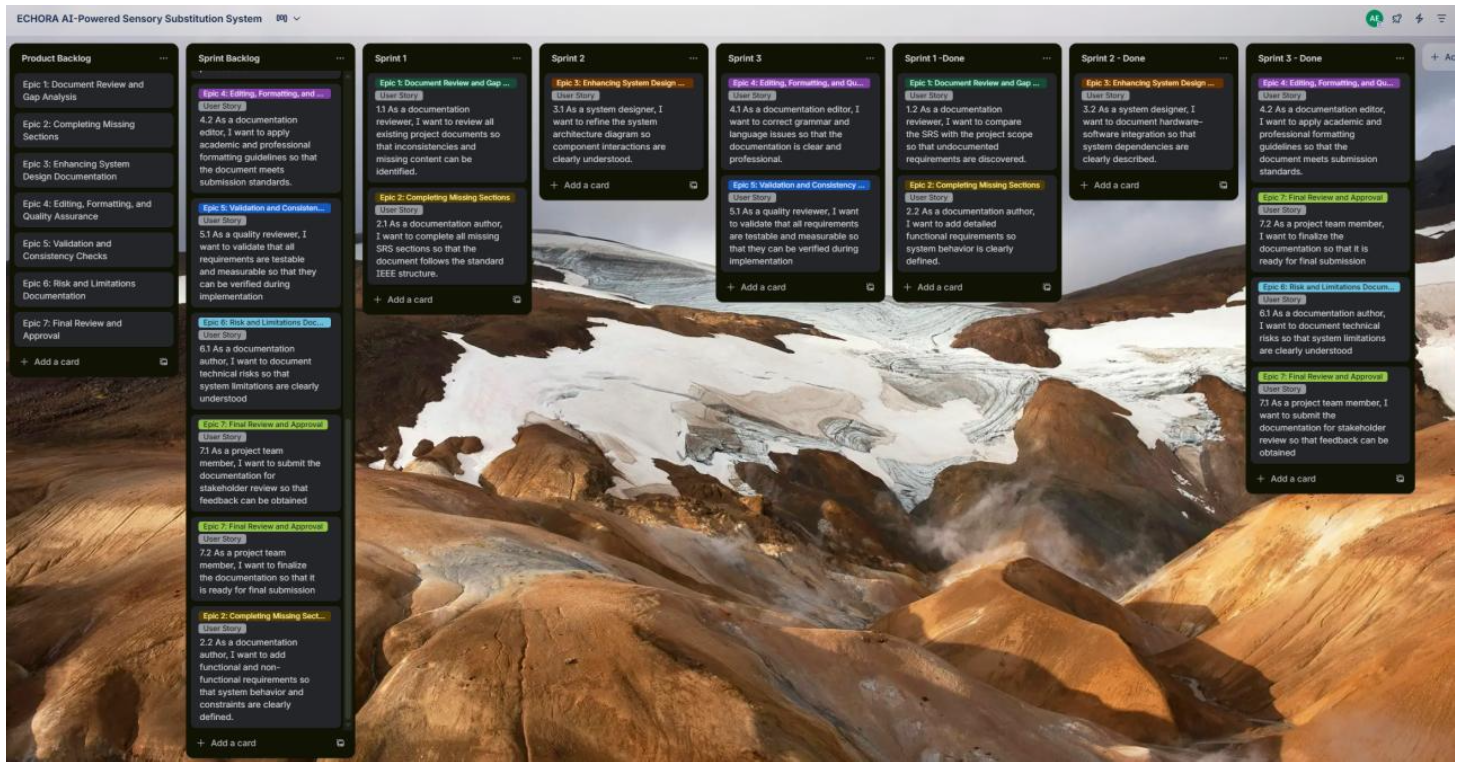
\includegraphics[height=0.6\textwidth]{assets/agile/trello doc phase.png}
\caption{Trello Backlog Documentation Phase}
\label{fig:agile_doc_trello}
\end{figure}

\begin{figure}[H]
\raggedright
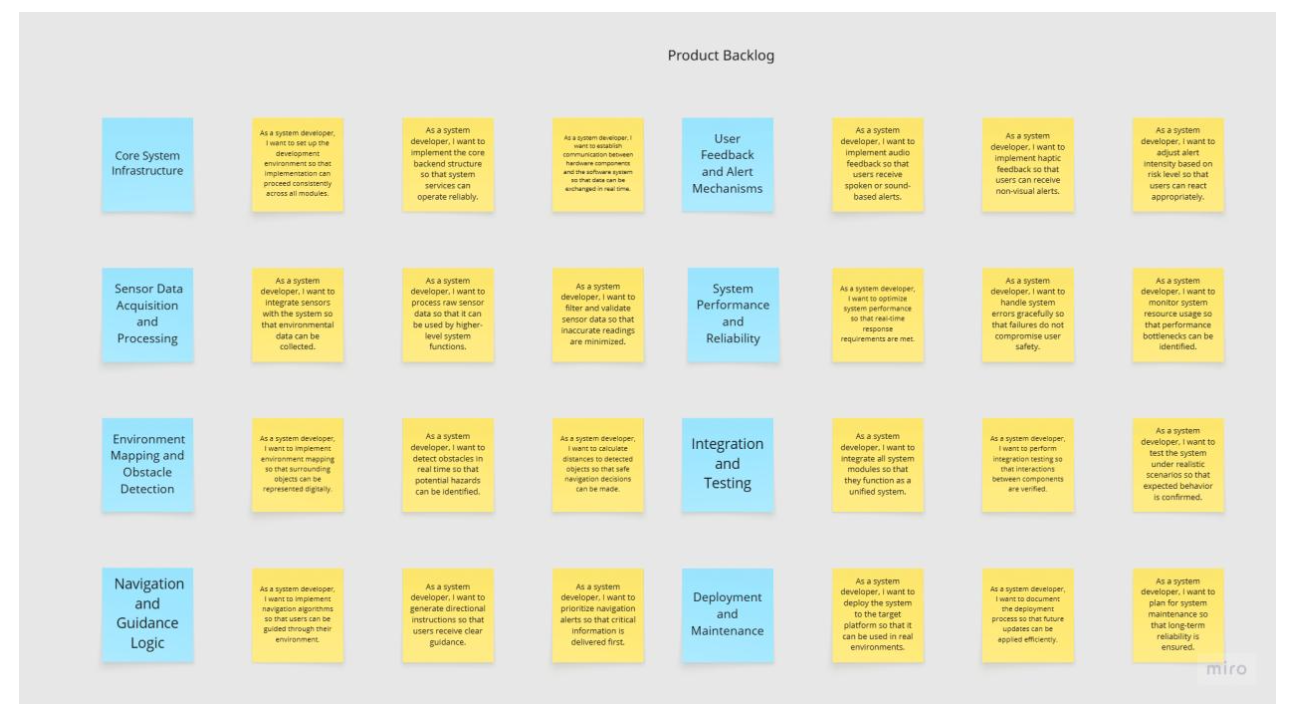
\includegraphics[height=0.6\textwidth]{assets/agile/imp phase.png}
\caption{Implementation Phase Backlog}
\label{fig:agile_impl_backlog}
\end{figure}

\begin{figure}[H]
\raggedright

\includegraphics[height=0.6\textwidth]{assets/agile/s1 impl phase.png}
\caption{Sprint 1 Implementation Phase}
\label{fig:agile_impl_s1}
\end{figure}

\begin{figure}[H]
\raggedright

\includegraphics[height=0.6\textwidth]{assets/agile/s2 impl phase.png}
\caption{Sprint 2 Implementation Phase}
\label{fig:agile_impl_s2}
\end{figure}

\begin{figure}[H]
\raggedright
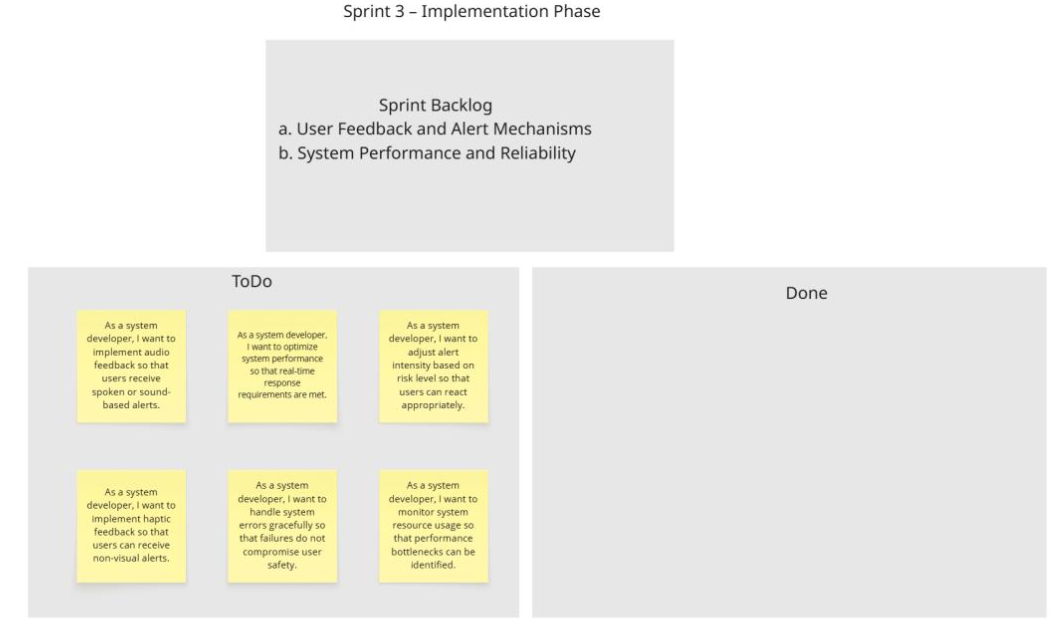
\includegraphics[height=0.6\textwidth]{assets/agile/s3 impl phase.png}
\caption{Sprint 3 Implementation Phase}
\label{fig:agile_impl_s3}
\end{figure}

\begin{figure}[H]
\raggedright

\includegraphics[height=0.6\textwidth]{assets/agile/s4 impl phase.png}
\caption{Sprint 4 Implementation Phase}
\label{fig:agile_impl_s4}
\end{figure}

\begin{figure}[H]
\raggedright
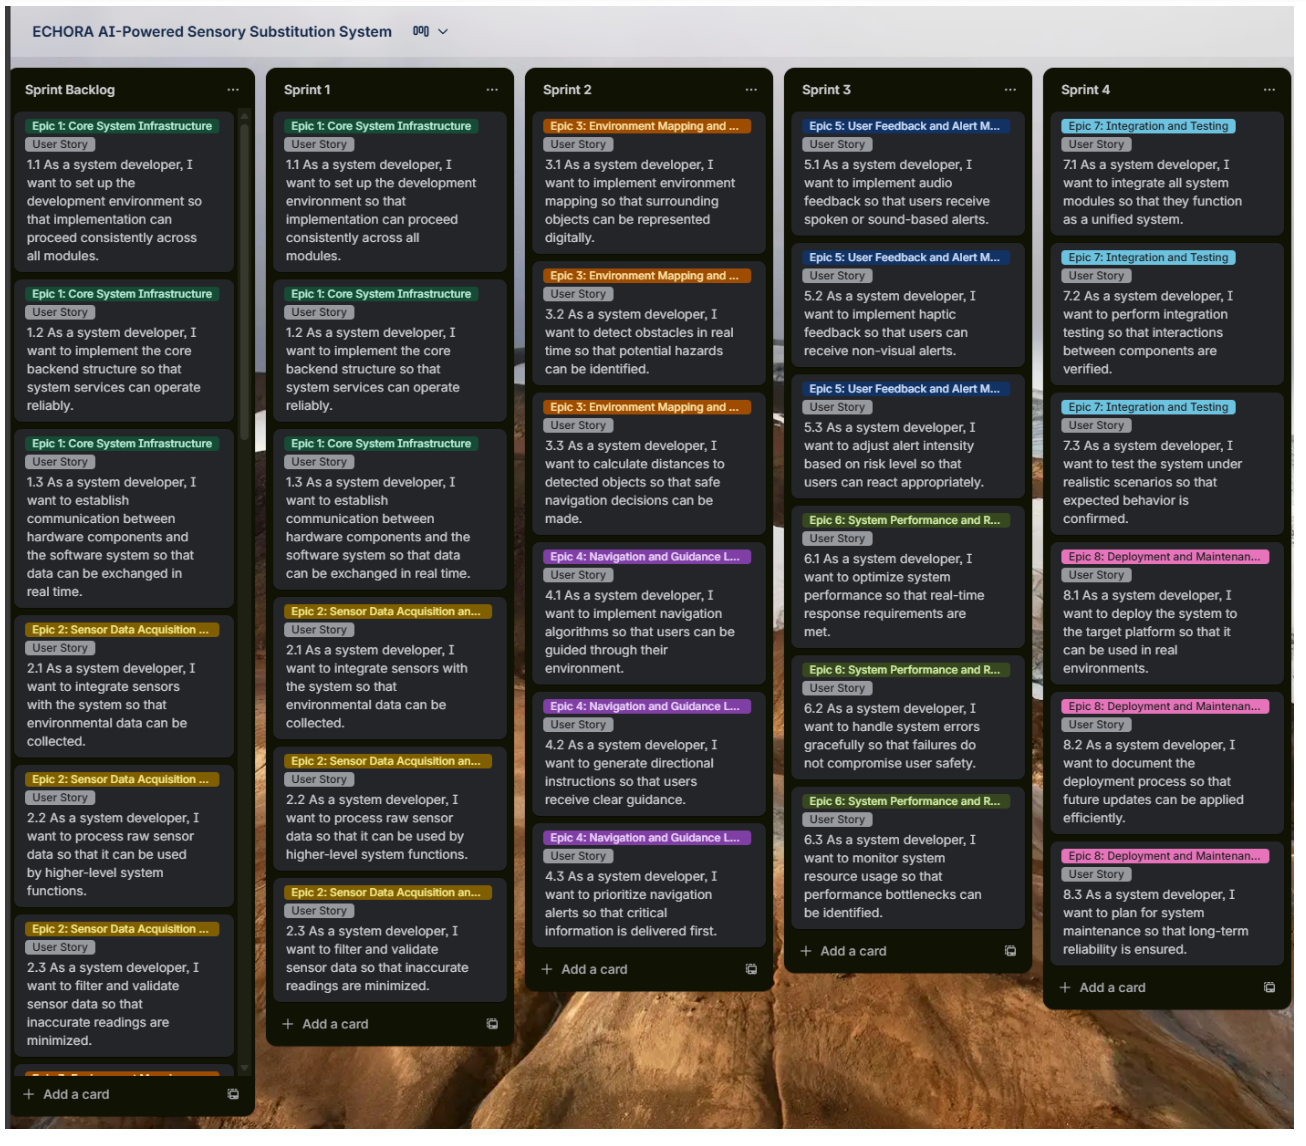
\includegraphics[height=1.0\textwidth]{assets/agile/trello impl phase.png}
\caption{Trello Backlog Implementation Phase}
\label{fig:agile_impl_trello}
\end{figure}
